\documentclass[tikz,crop,convert={density=200,outext=.png},border=0.4cm]{standalone}

\usepackage{pgfplots}
\usepackage{amsmath}
\usetikzlibrary{arrows.meta}
\usepackage{physics}
\usepackage{xcolor}
\definecolor{pow_1}{RGB}{103,0,31}
\pgfplotsset{compat=newest,
    %width=6cm,
    %height=3cm,
    scale only axis=true,
    max space between ticks=25pt,
    try min ticks=5,
    every axis/.style={
        axis y line=middle,
        axis x line=middle,
        axis line style={thick,->,>=latex, shorten >=-.3cm}
    },
    every axis plot/.append style={thick},
    tick style={black, thick},
}
\tikzset{
    semithick/.style={line width=0.8pt},
}
\usepgfplotslibrary{groupplots}
\usepgfplotslibrary{dateplot}
% Document begins
\begin{document}
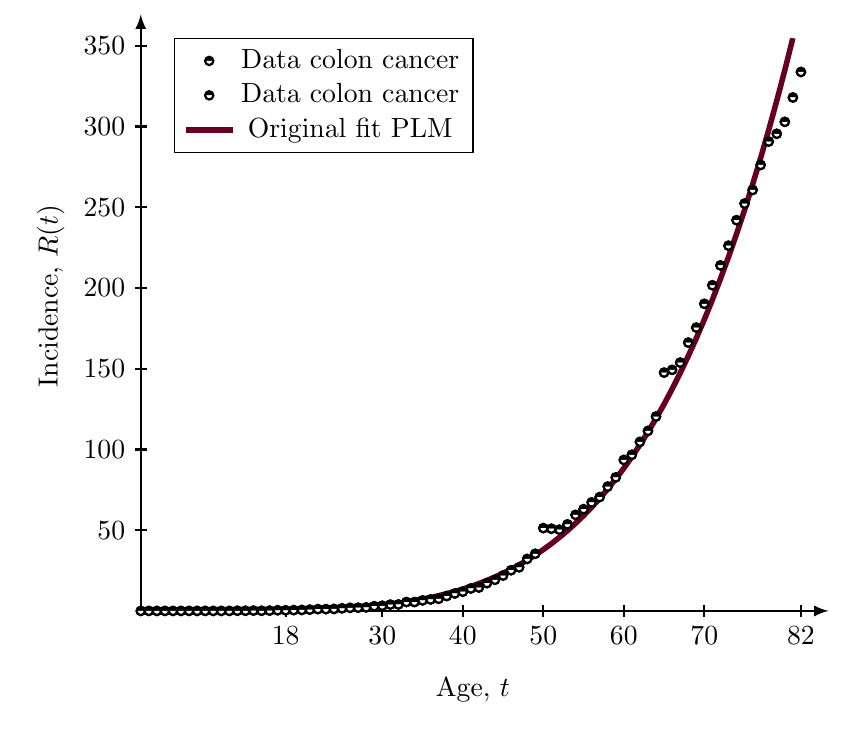
\begin{tikzpicture}
  % The axis of the plot
\begin{axis}[
    %title={Model: $\dv{y}{t}=\frac{2y}{t}$ with solution $y(t)=C_1t^2$\\Symmetry: $\Gamma_{\epsilon}=(t,y)\mapsto\left(\exp\left(\epsilon\right)t,\exp\left(-\epsilon\right)y\right)$},
    title style = {align=left},
    xlabel={Age, $t$},
    ylabel={Incidence, $R(t)$},
    %ylabel={Logarithm of Incidence, $\ln\left(R(t)\right)$},        
    x label style={at={(axis description cs:0.5,-0.1)},anchor=north},
    y label style={at={(axis description cs:-0.1,0.55)},rotate=90,anchor=south},    
    xmin=0, xmax=82.5,
    % xmin=-27, xmax=5,
    %ymin=-20, ymax=20,
    %xtick={-30,-27,...,9},
    xtick={0,18,30,40,...,60,70,82},    
    %ytick={-15,-10,...,15},
    legend style={at={(axis description cs:0.05,0.9)},anchor=west},    
    %legend pos=north west,
    %ymajorgrids=true,
    grid style=dashed,
]
% Plot the data
\addplot[
only marks, mark=halfcircle*,mark size=1.5pt,color=black,
]
coordinates {%
(0.0,0.0)
(1.0,0.0)
(2.0,0.0)
(3.0,0.0)
(4.0,0.0)
(5.0,0.0)
(6.0,0.0)
(7.0,0.0)
(8.0,0.0)
(9.0,0.0)
(10.0,0.0)
(11.0,0.0)
(12.0,0.1)
(13.0,0.1)
(14.0,0.2)
(15.0,0.1)
(16.0,0.2)
(17.0,0.4)
(18.0,0.4)
(19.0,0.5)
(20.0,0.6)
(21.0,0.8)
(22.0,1.1)
(23.0,1.1)
(24.0,1.2)
(25.0,1.6)
(26.0,1.9)
(27.0,2.0)
(28.0,2.2)
(29.0,2.9)
(30.0,3.2)
(31.0,3.9)
(32.0,4.0)
(33.0,5.5)
(34.0,5.5)
(35.0,6.5)
(36.0,7.1)
(37.0,7.5)
(38.0,9.2)
(39.0,10.8)
(40.0,11.9)
(41.0,13.9)
(42.0,14.5)
(43.0,17.2)
(44.0,19.3)
(45.0,21.9)
(46.0,25.2)
(47.0,27.0)
(48.0,32.2)
(49.0,35.4)
(50.0,51.3)
(51.0,50.9)
(52.0,50.3)
(53.0,53.6)
(54.0,59.5)
(55.0,63.0)
(56.0,67.2)
(57.0,70.5)
(58.0,77.0)
(59.0,82.7)
(60.0,93.5)
(61.0,96.7)
(62.0,104.7)
(63.0,111.5)
(64.0,120.4)
(65.0,147.6)
(66.0,149.3)
(67.0,153.8)
(68.0,166.2)
(69.0,175.5)
(70.0,190.2)
(71.0,201.7)
(72.0,214.0)
(73.0,226.2)
(74.0,242.0)
(75.0,252.3)
(76.0,260.7)
(77.0,276.2)
(78.0,290.7)
(79.0,295.5)
(80.0,302.9)
(81.0,318.0)
(82.0,333.8)
};
\addlegendentry{Data colon cancer}
\addplot[
only marks, mark=halfcircle*,mark size=1.5pt,color=black,
]
coordinates {%
(0.0,0.0)
(1.0,0.0)
(2.0,0.0)
(3.0,0.0)
(4.0,0.0)
(5.0,0.0)
(6.0,0.0)
(7.0,0.0)
(8.0,0.0)
(9.0,0.0)
(10.0,0.0)
(11.0,0.0)
(12.0,0.1)
(13.0,0.1)
(14.0,0.2)
(15.0,0.1)
(16.0,0.2)
(17.0,0.4)
(18.0,0.4)
(19.0,0.5)
(20.0,0.6)
(21.0,0.8)
(22.0,1.1)
(23.0,1.1)
(24.0,1.2)
(25.0,1.6)
(26.0,1.9)
(27.0,2.0)
(28.0,2.2)
(29.0,2.9)
(30.0,3.2)
(31.0,3.9)
(32.0,4.0)
(33.0,5.5)
(34.0,5.5)
(35.0,6.5)
(36.0,7.1)
(37.0,7.5)
(38.0,9.2)
(39.0,10.8)
(40.0,11.9)
(41.0,13.9)
(42.0,14.5)
(43.0,17.2)
(44.0,19.3)
(45.0,21.9)
(46.0,25.2)
(47.0,27.0)
(48.0,32.2)
(49.0,35.4)
(50.0,51.3)
(51.0,50.9)
(52.0,50.3)
(53.0,53.6)
(54.0,59.5)
(55.0,63.0)
(56.0,67.2)
(57.0,70.5)
(58.0,77.0)
(59.0,82.7)
(60.0,93.5)
(61.0,96.7)
(62.0,104.7)
(63.0,111.5)
(64.0,120.4)
(65.0,147.6)
(66.0,149.3)
(67.0,153.8)
(68.0,166.2)
(69.0,175.5)
(70.0,190.2)
(71.0,201.7)
(72.0,214.0)
(73.0,226.2)
(74.0,242.0)
(75.0,252.3)
(76.0,260.7)
(77.0,276.2)
(78.0,290.7)
(79.0,295.5)
(80.0,302.9)
(81.0,318.0)
(82.0,333.8)
};
\addlegendentry{Data colon cancer}

% Plot the model
\addplot[
color=pow_1,line width=2pt,
]
coordinates {%
(18.0,0.3345084990613453)
(19.0,0.4297021584856)
(20.0,0.5449390701407204)
(21.0,0.6831138934528704)
(22.0,0.8473673217256595)
(23.0,1.041093787018005)
(24.0,1.2679490309196324)
(25.0,1.5318575495141002)
(26.0,1.8370199199700064)
(27.0,2.187920015470079)
(28.0,2.5893321145555084)
(29.0,3.046327910411699)
(30.0,3.564283425139173)
(31.0,4.148885833628743)
(32.0,4.8061402012843875)
(33.0,5.542376139503835)
(34.0,6.364254382529409)
(35.0,7.278773289015399)
(36.0,8.293275271419025)
(37.0,9.415453156106716)
(38.0,10.653356476872272)
(39.0,12.01539770438695)
(40.0,13.510358413940704)
(41.0,15.147395393687345)
(42.0,16.936046695472793)
(43.0,18.886237630202576)
(44.0,21.008286709591786)
(45.0,23.31291153603875)
(46.0,25.811234642265422)
(47.0,28.514789282282525)
(48.0,31.435525175152826)
(49.0,34.58581420295202)
(50.0,37.97845606425686)
(51.0,41.626683884422505)
(52.0,45.544169783852006)
(53.0,49.7450304054052)
(54.0,54.24383240203751)
(55.0,59.05559788571353)
(56.0,64.19580983859026)
(57.0,69.68041748742559)
(58.0,75.52584164212143)
(59.0,81.74897999927721)
(60.0,88.3672124115879)
(61.0,95.39840612389858)
(62.0,102.86092097667111)
(63.0,110.77361457762355)
(64.0,119.15584744223477)
(65.0,128.0274881038156)
(66.0,137.4089181937961)
(67.0,147.32103749286378)
(68.0,157.785268953576)
(69.0,168.82356369501593)
(70.0,180.45840597008737)
(71.0,192.7128181059721)
(72.0,205.61036541829975)
(73.0,219.17516109953382)
(74.0,233.43187108206848)
(75.0,248.4057188765182)
(76.0,264.12249038567484)
(77.0,280.60853869454996)
(78.0,297.8907888369772)
(79.0,315.9967425391678)
(80.0,334.954482940638)
(81.0,354.7926792929032)
};
\addlegendentry{Original fit PLM}

\end{axis}
\end{tikzpicture}

\end{document}
